\subsection{Complete Methods under Practical Residual Channels}

All 627 registered readouts are complete: 528 newly trained external Full models, 66 PAMF supervised models, six new native-T1 models and 27 exact-contract native-T1 reuses. Each freezes two routes, three disjoint generalization populations and seven observations before independent scoring. The 600 new F models and four new eight-stage G lineages require no further training. We verify 742938 serialized confusion matrices and 371469 net-correction cells, reusing the previously verified F1/F2 overall cells. ManyRx uses ten classes and the other conditions six.

Table~\ref{tab:residual-f0} retains the complete channel/ordinary-PL four-cell comparison on the F0 cross-RX population. Channel augmentation is not uniformly beneficial, and ordinary PL does not consistently improve a complete baseline. Raw-F and restored performance are therefore reported together. G-L is used by A/C and supervised PAMF, whereas G-LU is used by B/D and native T1; restored PL-group differences include this additional G-data permission. PAMF-T1 retains its own selective self-training and original internal views, so comparison against ordinary-PL baselines concerns complete recipes, not one isolated SSL loss.

\begin{table*}[!t]\centering\footnotesize\setlength{\tabcolsep}{4pt}\renewcommand{\arraystretch}{1.12}

\caption{F0 cross-RX test (D1--D3; 126000 packets/view). Accuracy and Macro-F1 in percent, mean$\pm$sample SD over three F seeds. A/B/C/D denote channel off/on crossed with PL off/on. No CE-only baseline is included.}\label{tab:residual-f0}

\begin{tabular*}{\textwidth}{@{\extracolsep{\fill}}llrrrrr@{}}\toprule Method & Cell & Raw clean & Raw S6 & Restored clean & Restored S6 & Restored S6 F1\\\midrule

RIEI & A & \pmv{66.93}{0.71} & \pmv{52.43}{0.98} & \pmv{66.91}{0.69} & \pmv{62.43}{1.25} & \pmv{58.09}{1.49}\\

DRIFT-v2 & A & \pmv{66.21}{3.30} & \pmv{25.54}{1.08} & \pmv{66.18}{3.25} & \pmv{60.25}{2.60} & \pmv{60.75}{2.75}\\

IB-RFF & A & \pmv{66.29}{1.40} & \pmv{14.21}{3.49} & \pmv{66.29}{1.38} & \pmv{62.20}{0.64} & \pmv{61.89}{0.74}\\

SDG & A & \pmv{74.25}{0.88} & \pmv{56.08}{3.95} & \pmv{74.29}{0.88} & \pmv{66.81}{0.74} & \pmv{66.77}{0.69}\\

\addlinespace[2pt]

RIEI & B & \pmv{67.28}{0.88} & \pmv{52.70}{0.84} & \pmv{67.33}{0.93} & \pmv{63.01}{1.44} & \pmv{58.77}{1.88}\\

DRIFT-v2 & B & \pmv{67.69}{1.71} & \pmv{20.84}{1.57} & \pmv{67.64}{1.69} & \pmv{62.55}{2.23} & \pmv{62.97}{2.79}\\

IB-RFF & B & \pmv{66.44}{2.90} & \pmv{16.02}{2.91} & \pmv{66.47}{2.91} & \pmv{61.43}{1.79} & \pmv{61.00}{2.01}\\

SDG & B & \pmv{74.64}{0.14} & \pmv{57.01}{0.78} & \pmv{74.65}{0.13} & \pmv{68.48}{0.61} & \pmv{68.07}{0.46}\\

\addlinespace[2pt]

RIEI & C & \pmv{62.22}{1.53} & \pmv{50.08}{1.60} & \pmv{62.16}{1.49} & \pmv{57.59}{0.75} & \pmv{53.10}{0.85}\\

DRIFT-v2 & C & \pmv{61.77}{6.73} & \pmv{55.22}{5.28} & \pmv{61.71}{6.71} & \pmv{57.05}{4.48} & \pmv{56.10}{5.14}\\

IB-RFF & C & \pmv{66.74}{2.61} & \pmv{53.10}{1.83} & \pmv{66.77}{2.59} & \pmv{62.72}{1.74} & \pmv{62.37}{1.80}\\

SDG & C & \pmv{73.18}{2.16} & \pmv{65.16}{2.03} & \pmv{73.25}{2.16} & \pmv{66.46}{1.33} & \pmv{66.56}{1.33}\\

\addlinespace[2pt]

RIEI & D & \pmv{61.63}{1.89} & \pmv{49.95}{1.55} & \pmv{61.68}{1.85} & \pmv{56.73}{0.91} & \pmv{52.34}{1.27}\\

DRIFT-v2 & D & \pmv{66.12}{3.20} & \pmv{56.76}{2.29} & \pmv{66.11}{3.18} & \pmv{60.75}{4.42} & \pmv{58.46}{2.87}\\

IB-RFF & D & \pmv{66.63}{2.29} & \pmv{52.57}{2.17} & \pmv{66.65}{2.24} & \pmv{62.21}{2.86} & \pmv{61.74}{3.12}\\

SDG & D & \pmv{74.32}{1.52} & \pmv{65.30}{1.14} & \pmv{74.31}{1.50} & \pmv{67.12}{0.97} & \pmv{67.25}{1.09}\\

\addlinespace[2pt]

PAMF & A & \pmv{85.41}{0.74} & \pmv{44.42}{7.22} & \pmv{85.37}{0.76} & \pmv{77.13}{0.85} & \pmv{76.76}{0.95}\\

PAMF & C & \pmv{84.86}{0.80} & \pmv{71.96}{0.44} & \pmv{84.91}{0.74} & \pmv{76.48}{0.45} & \pmv{76.18}{0.52}\\

PAMF & Native T1 & \pmv{85.48}{0.87} & \pmv{71.53}{1.02} & \pmv{85.58}{0.92} & \pmv{78.21}{0.84} & \pmv{78.12}{0.85}\\

\bottomrule\end{tabular*}\end{table*}

\begin{figure*}[!t]\centering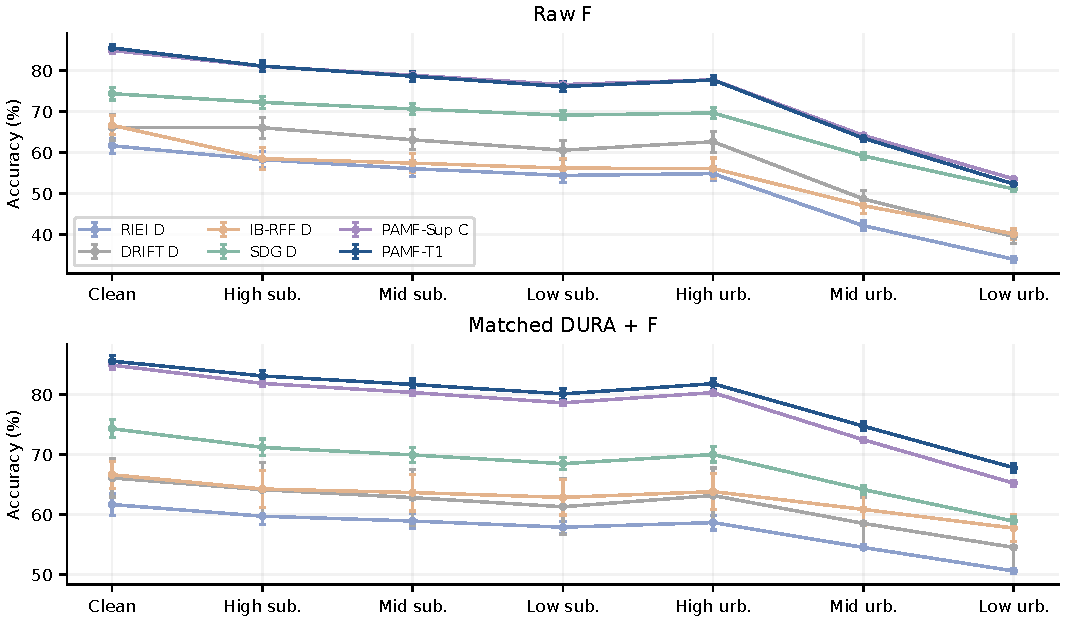
\includegraphics[width=.70\textwidth]{images/practical_full/F0_seven_views.pdf}\caption{F0 cross-RX accuracy on every frozen observation. External D uses the common residual-channel/ordinary-PL recipe; PAMF-Sup C uses its supervised residual-channel recipe and native T1 retains its fixed training method. This plot shows the matching DURA route; the accompanying independent direct-F figure is included in the reproducible figure kit. Error bars are three-F-seed SD.}\label{fig:residual-scenes}\end{figure*}

\subsubsection{Receiver and Date Generalization}

The new F1 and F2 source sets each replace four of the five F0 source receivers, and their pairwise source-set overlap is one. Table~\ref{tab:residual-generalization} separates earlier unseen-date evaluation on source RX, unseen RX on training dates, and their conjunction. Dates and receiver populations are not pooled. Native semi-supervision does not outperform the supervised recipe in every cell; all negative differences remain in the archive.

\begin{table*}[!t]\centering\footnotesize\setlength{\tabcolsep}{4pt}\renewcommand{\arraystretch}{1.12}

\caption{PAMF generalization after matching G (S6 accuracy, \%). Supervised A/C use G-L; native T1 uses G-LU. Each entry is the three-F-seed mean$\pm$SD.}\label{tab:residual-generalization}

\begin{tabular*}{\textwidth}{@{\extracolsep{\fill}}llrrr@{}}\toprule Split & PAMF recipe & Cross date & Cross RX & Cross date + RX\\\midrule

F0 & Supervised, channel off & \pmv{90.44}{0.26} & \pmv{77.13}{0.85} & \pmv{75.72}{0.11}\\

F0 & Supervised, channel on & \pmv{91.20}{0.16} & \pmv{76.48}{0.45} & \pmv{74.49}{0.97}\\

F0 & Native T1 & \pmv{91.93}{0.07} & \pmv{78.21}{0.84} & \pmv{75.95}{0.88}\\

\addlinespace[2pt]

F1 & Supervised, channel off & \pmv{83.43}{0.59} & \pmv{66.05}{0.92} & \pmv{66.31}{0.86}\\

F1 & Supervised, channel on & \pmv{83.04}{0.92} & \pmv{65.87}{0.50} & \pmv{65.47}{0.22}\\

F1 & Native T1 & \pmv{84.48}{0.95} & \pmv{66.96}{0.43} & \pmv{65.84}{0.11}\\

\addlinespace[2pt]

F2 & Supervised, channel off & \pmv{86.45}{0.08} & \pmv{75.16}{1.01} & \pmv{75.00}{0.84}\\

F2 & Supervised, channel on & \pmv{87.23}{0.49} & \pmv{74.22}{0.78} & \pmv{74.65}{1.14}\\

F2 & Native T1 & \pmv{88.52}{0.76} & \pmv{74.53}{0.15} & \pmv{74.49}{0.26}\\

\addlinespace[2pt]

\bottomrule\end{tabular*}\end{table*}

\subsubsection{Label Availability, ManyRx and Source Count}

Table~\ref{tab:residual-data} reports the one/five-percent training-label conditions, the default ten-percent condition and ManyRx. External rows use fixed D rather than selecting a cell from target scores. PAMF-Sup C and native T1 remain separate complete recipes. The source-count curves in Fig.~\ref{fig:residual-source} use m=1,2,3,4,6 with natural source budgets and the same six target RX: 108000 seen-date packets and 36000 D0 packets. No fixed-L budget or m=5 point is added; the seven-target F0 setting is not inserted into these curves.

\begin{table*}[!t]\centering\footnotesize\setlength{\tabcolsep}{4pt}\renewcommand{\arraystretch}{1.12}

\caption{Cross-RX S6 accuracy (\%) across dataset/label conditions. Columns give each condition separately; classes are six for ManySig and ten for ManyRx.}\label{tab:residual-data}

\begin{tabular*}{\textwidth}{@{\extracolsep{\fill}}lrrrrrrrr@{}}\toprule & \multicolumn{2}{c}{F0, 10\% L} & \multicolumn{2}{c}{F0, 1\% L} & \multicolumn{2}{c}{F0, 5\% L} & \multicolumn{2}{c}{ManyRx}\\

Method & Raw & G+F & Raw & G+F & Raw & G+F & Raw & G+F\\\midrule

RIEI D & \pmv{49.95}{1.55} & \pmv{56.73}{0.91} & \pmv{26.20}{8.61} & \pmv{33.99}{18.93} & \pmv{42.90}{4.07} & \pmv{41.11}{1.49} & \pmv{25.58}{1.98} & \pmv{28.70}{5.43}\\

DRIFT D & \pmv{56.76}{2.29} & \pmv{60.75}{4.42} & \pmv{17.39}{0.62} & \pmv{22.33}{2.03} & \pmv{35.73}{1.15} & \pmv{40.26}{8.18} & \pmv{34.09}{3.23} & \pmv{43.34}{3.64}\\

IB-RFF D & \pmv{52.57}{2.17} & \pmv{62.21}{2.86} & \pmv{45.27}{3.63} & \pmv{64.34}{2.47} & \pmv{51.83}{0.65} & \pmv{61.69}{0.97} & \pmv{48.59}{2.74} & \pmv{64.99}{0.77}\\

SDG D & \pmv{65.30}{1.14} & \pmv{67.12}{0.97} & \pmv{62.34}{0.08} & \pmv{68.31}{1.09} & \pmv{63.62}{1.48} & \pmv{67.06}{0.94} & \pmv{61.40}{0.54} & \pmv{66.07}{0.75}\\

PAMF-Sup C & \pmv{71.96}{0.44} & \pmv{76.48}{0.45} & \pmv{68.83}{1.10} & \pmv{69.26}{0.21} & \pmv{70.98}{0.54} & \pmv{74.51}{0.47} & \pmv{64.56}{0.13} & \pmv{71.40}{0.50}\\

PAMF-T1 & \pmv{71.53}{1.02} & \pmv{78.21}{0.84} & \pmv{70.59}{0.12} & \pmv{74.04}{0.73} & \pmv{71.33}{0.49} & \pmv{75.99}{0.69} & \pmv{63.54}{0.39} & \pmv{72.59}{0.22}\\

\bottomrule\end{tabular*}\end{table*}

\begin{figure*}[!t]\centering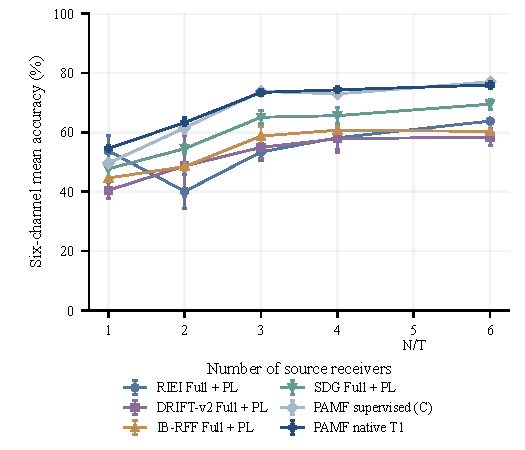
\includegraphics[width=.70\textwidth]{images/practical_full/source_count.pdf}\caption{Matching-DURA cross-RX natural-budget source-count curves, with fixed six-target populations and the same preregistered recipes as Table~\ref{tab:residual-data}. Scenes average within seed before the three-seed SD. Decreases and method-rank changes are retained.}\label{fig:residual-source}\end{figure*}

The 600 new F models sum to 246.37 shared-worker elapsed hours; 27 reused F sources contribute 46.26 historical hours. Four new complete G lineages sum to 18.42 hours; the 17 other fully timed G lineages sum to 89.26 historical hours. Original fixed-F0 G-LU ancestor timings remain incomplete. The 3811 unique CPU augmentation-cache productions sum to 1.52 elapsed hours, the 22 restored-IQ caches to 1.17 hours and cached F predictions to 21.67 shared-worker hours. These are not exclusive GPU hours, CPU core-hours, online G+F latency or an end-to-end speedup. We retain all external augmentation/PL counts, including 61 zero-acceptance training rows. Complete native-PAMF gate acceptance and per-F realized channel counts are not recoverable from the compact telemetry and are left missing.

The following PAMF mechanism studies retain their original F0 all-target-date population (168000 packets/view). They are independently frozen historical mechanism evidence, not relabeled as the 126000-packet cross-RX endpoint above. Existing mechanism and timing measurements are reused without retraining or retesting.
